%!TEX root = document.tex

%%%%%%%%%%%%%%%%%%%%%%%%%%%%%%%%%%%%%%%%%%%%%%%%%%%%%%%%%%%%%%%%%%%%%%%%%%%
\begin{figure*}[tbp!]
%\centering
\hspace{-8mm}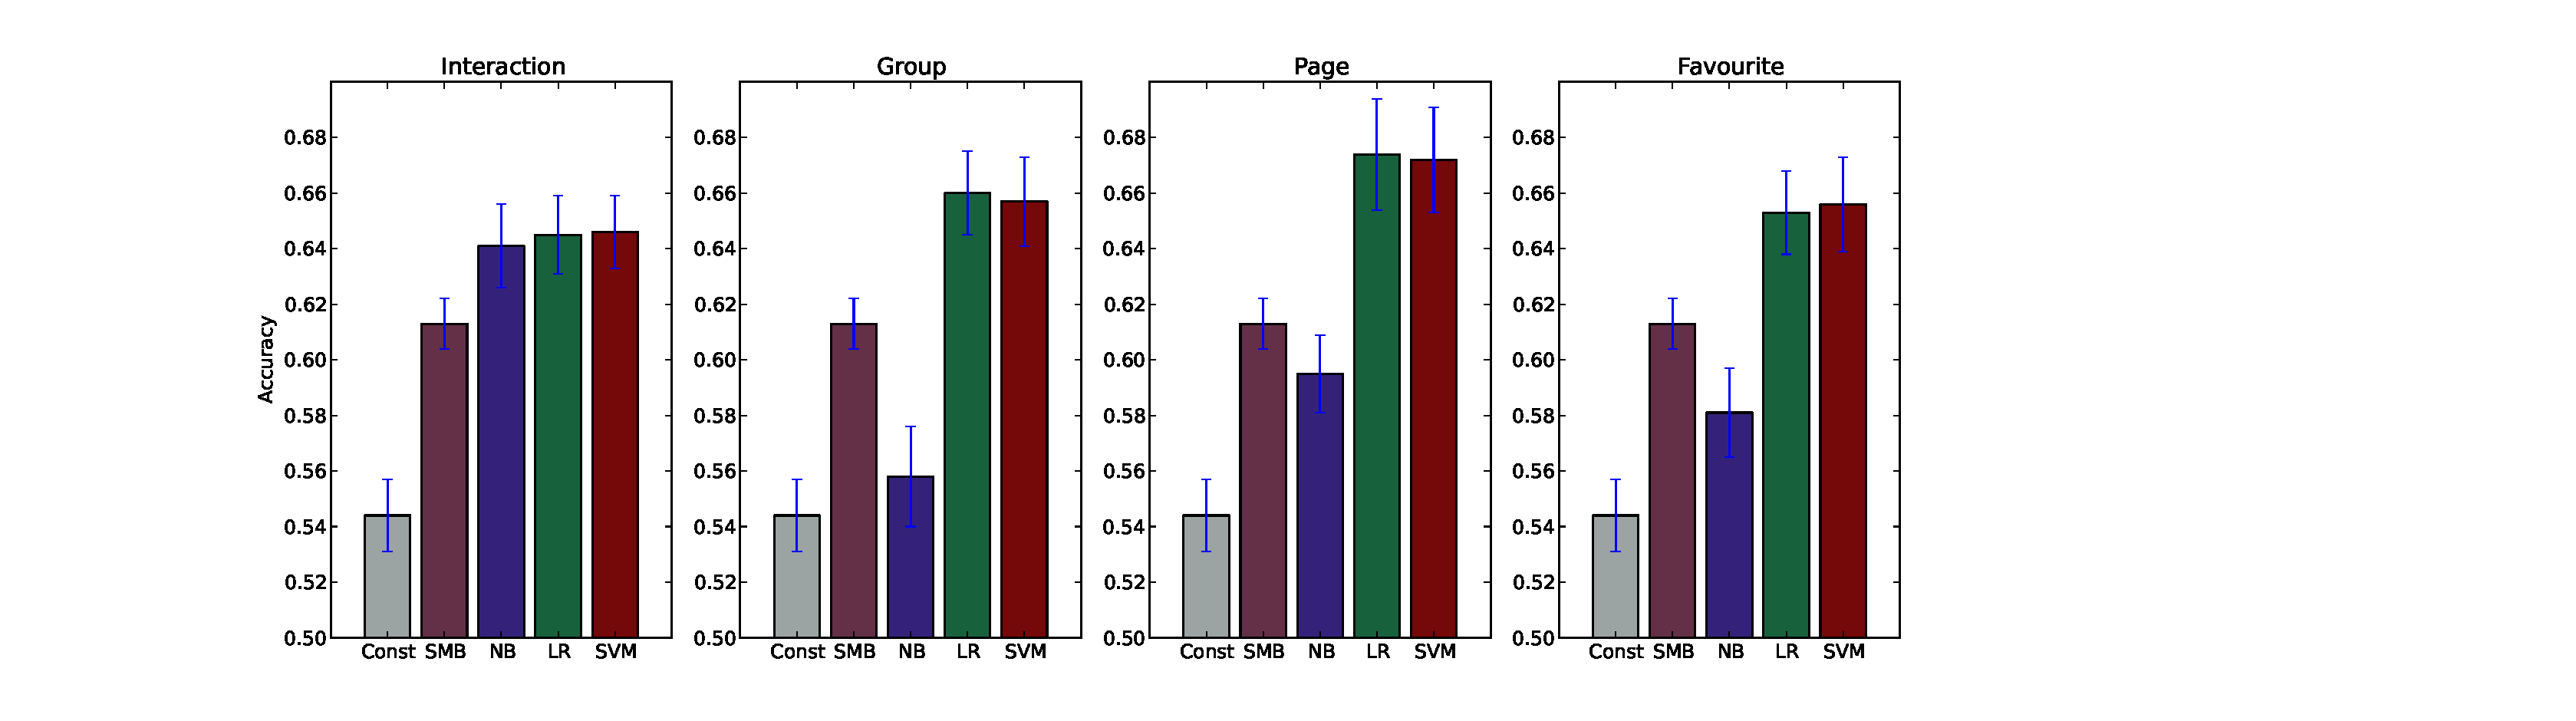
\includegraphics[width=230mm]{data/plots/accuracy/accuracy.eps}
\caption{ Accuracy of predictors (constant, social matchbox, naive bayes, logistic regression, SVM) for Interaction and Activity  features }
\label{Fig1}
\end{figure*}
%%%%%%%%%%%%%%%%%%%%%%%%%%%%%%%%%%%%%%%%%%%%%%%%%%%%%%%%%%%%%%%%%%%%%%%%%%%

\section{Social Affinity filtering}

%Social affinity filtering (SAF) is based on the idea that affinity
%between users expressed in social networks via interactions and
%activities is predictive of user preferences.  
Social affinity group and the associated features defined in Sec~\ref{ssec:SAfeature} 
are used to build predictors for $\likes(u,i)$ given features $X$.
%as follows: a classifier takes a user $u$ and item $i$ and must predict
%whether $\likes(u,i)$ given features that can be derived from the
%social network.  
In SAF, these features are the boolean
variables $X_{k,u,i}$ indicating whether any users in the $k$th SAG of
user $u$ also liked $i$.  For example, $k$ could be the SAG of $u$ for
the interaction of $\textit{link-like-incoming}$ or the activity of
liking the {\em Obama Re-Election Headquarters} Facebook page.  Then knowing whether
anyone in each SAG $k$ for user $u$ likes item $i$ provides a rich set
of fine-grained features for prediction.  It is up to SAF to learn how
to weight each SAG to aggregate their preferences into one final
prediction, which is done by training on historical data.

Formally, given a user $u$ and item $i$, a SAF classifier is a
function: $f: \x \to y$ where $y \in \{ \like, \dislike \}$ and $\x =
\langle u,i,x_1,\ldots,x_k \rangle$ where $x_j \in X_j$ ($1 \leq j
\leq k$) as previously formally defined in the Methodology.  To train $f$, one
simply provides a dataset of historical observations $D = \{ \langle
\x,y \rangle \}$, e.g., $f$ could be a linear classifier trained by an
SVM, logistic regression, or na\"{i}ve Bayes.  Then for future
predictions, we simply are given $\x$ and we ask the SAF classifier to
predict $y = f(\x)$.

Fig \ref{Fig1} compares the accuracies of constant predictor and
social matchbox with SAF based on na\"{i}ve Bayes, logistic regression
and SVM classification for a range of interaction and activity (group,
page, favourite) SAGs.  In all of our experiments SAF variants
performed significantly better than Social Matchbox and the constant
predictor except for na\"{i}ve Bayes, we conjecture this is due to the
correlations between SAGs that cause na\"{i}ve Bayes to over- or
under-estimate the true probability of likes.

In general we note in Fig \ref{Fig1} that activities appear to be
more predictive than interactions, but we believe the reasons for this
are quite simple: Interaction SAGs can only evaluate the friends of
user $u$ whereas Activity SAGs are able to look at all users,
independent of $u$'s friends.
Hence, given the general sparsity of ``likes'' data in Facebook, 
Activity SAGs appear to draw on a much larger group of SAGs
with much more activity.

Among activities, Fig \ref{Fig1} shows that activities are more
predictive than interactions. Among the activities, page likes are the
most predictive followed by group membership and favourites.
Returning to our conjecture that data sparsity can hurt SAF, we note
from Table~\ref{tab:interests} that page likes are more prevalent than
groups and favourites.  Moreover, these results may indicate that
there is more social affinity between co-members of inherently social
activities like groups and pages than between users who simply have
favourites in common.

Comparing SAF to the state-of-the-art in social
collaborative filtering (SCF) as represented by Social
Matchbox~\cite{Noel2012NOF}, we observe that SAF consistently
outperforms it.  We note that the key difference of SAF vs. SCF is
that SAF exploits the predictiveness of fine-grained interactions ---
it breaks down into groups, whereas most SCF
approaches~\cite{Noel2012NOF,lla,socinf,sr,rrmf,sorec,ste} is that
instead of collapsing a diverse set of interactions into aggregate
statistics such as the number of interactions between user $u_1$ and
user $u_2$, regardless of whether $u_1$ tagged $u_2$ in a photo or
$u_1$ liked a photo on $u_2$'s wall.  Clearly there is a great deal of
benefit deriving from the fine-grained interactions indicating why
without modeling any latent space and using a simple linear
classifier, SAF can outperform SCF methods based on matrix
factorization approaches that attempt to learn latent user and item
features.

On two final notes, we remark that SAF yields a computational and
optimization advantage over SCF in that it is straightforward and
efficient to find a globally optimal classifier with respect to certain training
criteria (e.g., optimising log loss in logistic regression or hinge
loss in SVMs) unlike SCF approaches that generally rely on
computationally expensive matrix factorization techniques that lack
optimality guarantees.  Further, we also note quite surprisingly that
SAF inherently scales to a large number of users and generalizes to
completely new users without suffering from the cold-start problem:
this is simply because nothing SAF learns is user dependent, it learns
to weight SAGs independent of any particular user.

Given the clearly demonstrated benefits of SAF, we now proceed in the
next two sections to analyse the two primary types of SAG features
(interactions and activities) to better understand characteristics of
both informative and uninformative SAGs in each context and the social
phenomena that may be responsible for these characteristics.
